\documentclass[12pt]{article}

\usepackage[margin=1in]{geometry}
\usepackage{amsmath,amsthm,amssymb}

\usepackage{graphicx}
\graphicspath{ {./assets/} }

\usepackage{algpseudocode}
\usepackage{algorithm}

\usepackage{tikz}

\newcommand{\wip}{\textbf{(WIP) }}
\newcommand{\tba}{\textbf{(TBA) }}

\newcommand{\blah}{\textbf{blah blah blah}}

\newcommand{\dsa}[1]{\textbf{[DSA: #1]}}

\begin{document}

\title{Project 1 — Report}
\author{
  Diogo Antunes\\
  99210
  \and
  Javier María\\
  99240
  \and
  Tomás Silva\\
  98973
}

\maketitle

\section*{Exercise 1}

The first exercise was to solve the CNF-SAT $\phi$ formula with the following constraints:

\begin{align}
        & (\lnot p_{1} \vee p_{3} \vee p_{4} \vee p_{5}) \\
        & (\lnot p_{3} \vee p_{4} \vee p_{5}) \\
        & (\lnot p_{1} \vee p_{3} \vee \lnot p_{4}) \\
        & (p_{1} \vee p_{2}) \\
        & (p_{1} \vee \lnot p_{2}) \\
        & (\lnot p_{1} \vee \lnot p_{5}) \\
        & (\lnot p_{3} \vee \lnot p_{4} \vee p_{5})
\end{align}

\vspace{0.5cm}

This was done using CDCL with 1-UIP (Unit Implication Point) as the conflict analysis strategy.
When going through conflict clauses, if a clause with only one literal that is assigned at the current level is encountered, then the 1-UIP has been found.
In this can, there's a backtrack to the variable with a largest decision level other than the current.

\vspace{0.5cm}

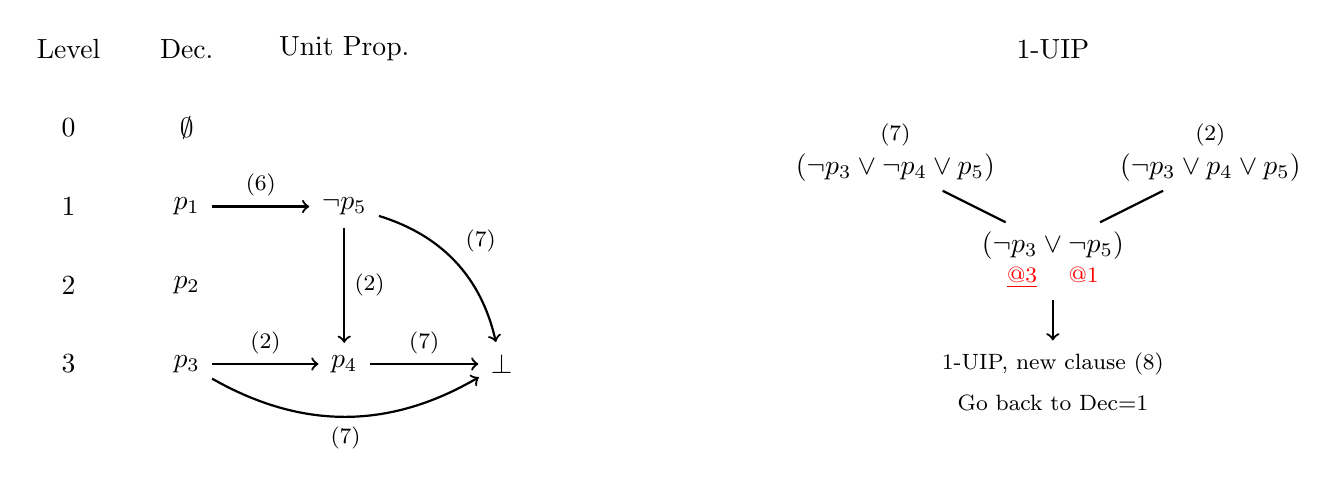
\begin{tikzpicture}[
    every node/.style={anchor=center},
    level/.style={anchor=center},
    decision/.style={anchor=center},
    unit/.style={anchor=center},
    clause/.style={anchor=center},
    arrow/.style={->, thick, shorten >=1pt, shorten <=1pt}
    ]

% Level and Decisions
\node[level] (Level Label) at (0,0) {Level};
\node[level] (Level 0) at (0,-1) {0};
\node[level] (Level 1) at (0,-2) {1};
\node[level] (Level 2) at (0,-3) {2};
\node[level] (Level 3) at (0,-4) {3};

\node[decision] at (1.5,0) {Dec.};
\node[decision] at (1.5,-1) {$\emptyset$};
\node[decision] (p1) at (1.5,-2) {$p_{1}$};
\node[decision] (p2) at (1.5,-3) {$p_{2}$};
\node[decision] (p3) at (1.5,-4) {$p_{3}$};

% Unit Propagation Column
\node[unit] at (3.5,0) {Unit Prop.};

\node[unit] (p5) at (3.5,-2) {$\lnot p_{5}$};
\node[unit] (p4) at (3.5,-4) {$p_{4}$};
\node[unit] (contra) at (5.5, -4) {$\bot$};

% Arrows for Unit Propagation
\draw[arrow] (p1) to node[midway, above] {\footnotesize (6)} (p5);
\draw[arrow] (p3) to node[midway, above] {\footnotesize (2)} (p4);
\draw[arrow] (p5) to node[midway, right] {\footnotesize (2)} (p4);
\draw[arrow] (p4) to node[midway, above] {\footnotesize (7)} (contra);
\draw[arrow, bend right] (p3) to node[midway, below] {\footnotesize (7)} (contra);
\draw[arrow, bend left] (p5) to node[midway, above right] {\footnotesize (7)} (contra);

% Conflict Analysis
\node[clause] (1-UIP Label) at (12.5,0) {1-UIP};
\node[clause] (c7) at (10.5,-1.5) {$(\lnot p_{3} \vee \lnot p_{4} \vee p_{5})$};
\node[above=0.15cm] at (c7) {\footnotesize (7)};
\node[clause] (c2) at (14.5,-1.5) {$(\lnot p_{3} \vee p_{4} \vee p_{5})$};
\node[above=0.15cm] at (c2) {\footnotesize (2)};
\node[clause] (d1) at (12.5,-2.5) {$(\lnot p_{3} \vee \lnot p_{5})$};
\node[below=0.15cm] (levels) at (d1) {\color{red} \footnotesize \underline{@3} \hspace{0.2cm} {@1}};
\node[clause, label={[align=center]below: \footnotesize Go back to Dec=1}] (expl) at (12.5,-4) {\footnotesize 1-UIP, new clause (8)};

% Arrows for conflict analysis
\draw[-, thick] (c7) to (d1);
\draw[-, thick] (c2) to (d1);
\draw[arrow] (levels) to (expl);

\end{tikzpicture}

\vspace{0.5cm}

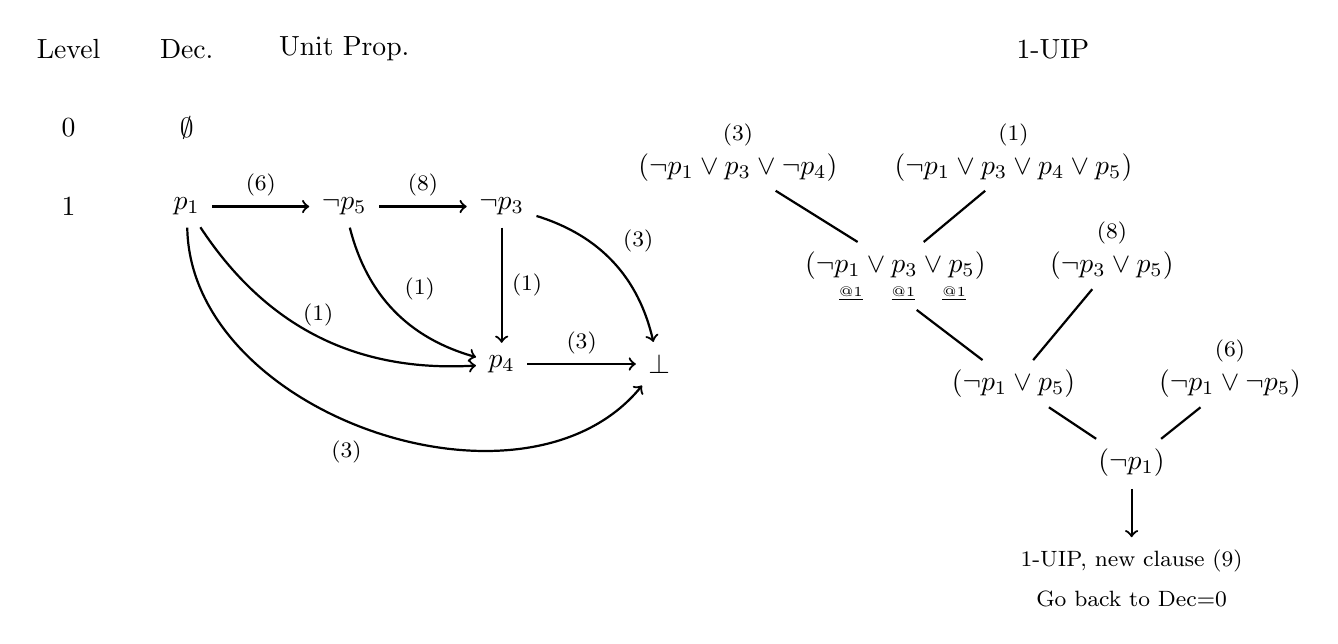
\begin{tikzpicture}[
    every node/.style={anchor=center},
    level/.style={anchor=center},
    decision/.style={anchor=center},
    unit/.style={anchor=center},
    clause/.style={anchor=center},
    arrow/.style={->, thick, shorten >=1pt, shorten <=1pt}
    ]

% Level and Decisions
\node[level] (Level Label) at (0,0) {Level};
\node[level] (Level 0) at (0,-1) {0};
\node[level] (Level 1) at (0,-2) {1};

\node[decision] at (1.5,0) {Dec.};
\node[decision] at (1.5,-1) {$\emptyset$};
\node[decision] (p1) at (1.5,-2) {$p_{1}$};

% Unit Propagation Column
\node[unit] at (3.5,0) {Unit Prop.};

\node[unit] (p5) at (3.5,-2) {$\lnot p_{5}$};
\node[unit] (p3) at (5.5,-2) {$\lnot p_{3}$};
\node[unit] (p4) at (5.5,-4) {$p_{4}$};
\node[unit] (contra) at (7.5, -4) {$\bot$};

% Arrows for Unit Propagation
\draw[arrow] (p1) to node[midway, above] {\footnotesize (6)} (p5);
\draw[arrow] (p5) to node[midway, above] {\footnotesize (8)} (p3);
\draw[arrow, bend right] (p1) to node[midway, above] {\footnotesize (1)} (p4);
\draw[arrow] (p3) to node[midway, right] {\footnotesize (1)} (p4);
\draw[arrow, bend right] (p5) to node[midway, above right] {\footnotesize (1)} (p4);
\draw[arrow, bend left] (p3) to node[midway, above right] {\footnotesize (3)} (contra);
\draw[arrow] (p4) to node[midway, above] {\footnotesize (3)} (contra);
\draw[arrow, bend right=70] (p1) to node[midway, below left] {\footnotesize (3)} (contra);

% Conflict Analysis
\node[clause] (1-UIP Label) at (12.5,0) {1-UIP};
\node[clause] (c3) at (8.5,-1.5) {$(\lnot p_{1} \vee p_{3} \vee \lnot p_{4})$};
\node[above=0.15cm] at (c3) {\footnotesize (3)};
\node[clause] (c1) at (12,-1.5) {$(\lnot p_{1} \vee p_{3} \vee p_{4} \vee p_{5})$};
\node[above=0.15cm] at (c1) {\footnotesize (1)};
\node[clause] (c8) at (13.25, -2.75) {$(\lnot p_{3} \vee p_{5})$};
\node[above=0.15cm] at (c8) {\footnotesize (8)};
\node[clause] (c6) at (14.75, -4.25) {$(\lnot p_{1} \vee \lnot p_{5})$};
\node[above=0.15cm] at (c6) {\footnotesize (6)};
\node[clause] (d1) at (10.5,-2.75) {$(\lnot p_{1} \vee p_{3} \vee p_{5})$};
\node[below=0.15cm] (levels) at (d1) {\tiny \hspace{0.1cm} \underline{@1} \hspace{0.2cm} \underline{@1} \hspace{0.18cm} \underline{@1}};
\node[clause] (d2) at (12,-4.25) {$(\lnot p_{1} \vee p_{5})$};
\node[clause] (d3) at (13.5,-5.25) {$(\lnot p_{1})$};

\node[clause, label={[align=center]below: \footnotesize Go back to Dec=0}] (expl) at (13.5,-6.5) {\footnotesize 1-UIP, new clause (9)};

% Arrows for conflict analysis
\draw[-, thick] (c3) to (d1);
\draw[-, thick] (c1) to (d1);
\draw[-, thick] (levels) to (d2);
\draw[-, thick] (c8) to (d2);
\draw[-, thick] (d2) to (d3);
\draw[-, thick] (c6) to (d3);
\draw[arrow] (d3) to (expl);

\end{tikzpicture}

\vspace{1cm}

\begin{tikzpicture}[
    every node/.style={anchor=center},
    level/.style={anchor=center},
    decision/.style={anchor=center},
    unit/.style={anchor=center},
    clause/.style={anchor=center},
    arrow/.style={->, thick, shorten >=1pt, shorten <=1pt}
    ]

% Level and Decisions
\node[level] (Level Label) at (0,0) {Level};
\node[level] (Level 0) at (0,-1) {0};

\node[decision] at (1.5,0) {Dec.};
\node[decision] (empty) at (1.5,-1) {$\emptyset$};

% Unit Propagation Column
\node[unit] at (3.5,0) {Unit Prop.};

\node[unit] (p1) at (3.5,-1) {$\lnot p_{1}$};
\node[unit] (p2) at (5.5,-1) {$p_{2}$};
\node[unit] (contra) at (5.5, -3) {$\bot$};

% Arrows for Unit Propagation
\draw[arrow] (empty) to node[midway, above] {\footnotesize (9)} (p1);
\draw[arrow] (p1) to node[midway, above] {\footnotesize (4)} (p2);
\draw[arrow, bend right] (p1) to node[midway, above right] {\footnotesize (5)} (contra);
\draw[arrow] (p2) to node[midway, right] {\footnotesize (5)} (contra);

% Conflict Analysis
\node[clause] (1-UIP Label) at (12,0) {1-UIP};
\node[clause] (c5) at (9.5,-1.5) {$(p_{1} \vee \lnot p_{2})$};
\node[above=0.15cm] at (c5) {\footnotesize (5)};
\node[clause] (c4) at (12,-1.5) {$(p_{1} \vee p_{2})$};
\node[above=0.15cm] at (c4) {\footnotesize (4)};
\node[clause] (c9) at (14.5, -1.5) {$(\lnot p_{1})$};
\node[above=0.15cm] at (c9) {\footnotesize (9)};
\node[clause] (d1) at (10.5, -2.75) {$(p_{1})$};
\node[clause] (d2) at (12, -4.25) {$\bot$};

\node[clause] (expl) at (12,-5.5) {\footnotesize Derived $\emptyset \implies$ UNSAT};

% Arrows for conflict analysis
\draw[-, thick] (c5) to (d1);
\draw[-, thick] (c4) to (d1);
\draw[-, thick] (d1) to (d2);
\draw[-, thick] (c9) to (d2);
\draw[arrow] (d2) to (expl);

\end{tikzpicture}

\vspace{1cm}

As it can be seen from the previous CDCL decision graphs, the formula $\phi$ is unsatisfiable.

\section*{Exercise 2}

The second exercise was to encode the nonogram puzzle as a SAT problem.
Two different encodings were implemented and tested.
Both follow the same structure -- encoding the puzzle is reduced to encoding a single line (row or column).

The first encoding is a ``brute-force'' approach that considers all possible placements of black squares in a given line.
Consecutive black squares will be called a \textit{gap} hereinafter.

The second encoding avoids the combinatorial blow-up in the number of possible configurations by directly expressing the rules of the puzzle as SAT constraints.

Both approaches proved to be useful because, despite being slower, the brute-force approach is easier to reason about and was used to debug the more efficient one.

\subsection*{Reduction to encoding a single line}

As was mentioned before, encoding the nonogram puzzle is reduced to encoding a single line.
In particular, the enconding of the puzzle will be the conjunction of the encodings of each row and column.

Formally, a line is a list of naturals $l = [g_j, \ldots, g_{j'}]$ and a puzzle is a tuple $\langle H, V\rangle$, where both $H$ and $V$ are a list of lines.
The encoding of a line $l = [g_j, \ldots, g_{j'}]$ of size $s$ is denoted $E(l, s)$ -- the two approaches differ in $E$'s definition.
The encoding of the entire puzzle is

\begin{center}
  $\bigwedge\limits_{l \in H} E(l, |V|) \wedge \bigwedge\limits_{l \in V} E(l, |H|)$
\end{center}


\subsection*{``Brute-force'' approach}

As was briefly mentioned before, the first and simpler approach to encode a single line is to consider all the possible placements of the gaps on a given line.
For instance, if $l = [1, 2]$ for a line of size 5, the possible configurations are the following:

\begin{center}

\begin{tikzpicture}
    % X _ X X _
    \foreach \x in {1,2,...,5} {
        \ifnum\x=1 \filldraw[fill=black] (\x*0.5, 0) rectangle (\x*0.5+0.5, -0.5);
        \else\ifnum\x=3 \filldraw[fill=black] (\x*0.5, 0) rectangle (\x*0.5+0.5, -0.5);
        \else\ifnum\x=4 \filldraw[fill=black] (\x*0.5, 0) rectangle (\x*0.5+0.5, -0.5);
        \else \draw (\x*0.5, 0) rectangle (\x*0.5+0.5, -0.5);
        \fi\fi\fi
    }

    % X _ _ X X
    \begin{scope}[shift={(3.5, 0)}]
    \foreach \x in {1,2,...,5} {
        \ifnum\x=1 \filldraw[fill=black] (\x*0.5, 0) rectangle (\x*0.5+0.5, -0.5);
        \else\ifnum\x=4 \filldraw[fill=black] (\x*0.5, 0) rectangle (\x*0.5+0.5, -0.5);
        \else\ifnum\x=5 \filldraw[fill=black] (\x*0.5, 0) rectangle (\x*0.5+0.5, -0.5);
        \else \draw (\x*0.5, 0) rectangle (\x*0.5+0.5, -0.5);
        \fi\fi\fi
    }
    \end{scope}

    % _ X _ X X
    \begin{scope}[shift={(7, 0)}]
    \foreach \x in {1,2,...,5} {
        \ifnum\x=2 \filldraw[fill=black] (\x*0.5, 0) rectangle (\x*0.5+0.5, -0.5);
        \else\ifnum\x=4 \filldraw[fill=black] (\x*0.5, 0) rectangle (\x*0.5+0.5, -0.5);
        \else\ifnum\x=5 \filldraw[fill=black] (\x*0.5, 0) rectangle (\x*0.5+0.5, -0.5);
        \else \draw (\x*0.5, 0) rectangle (\x*0.5+0.5, -0.5);
        \fi\fi\fi
    }
    \end{scope}
\end{tikzpicture}
\end{center}

Given the constraints of the puzzle, there are positions on the line that a given gap cannot start at.
To rule out the impossible starting positions, it will be useful to define the minimum and maximum start positions for a gap $i$.

\begin{center}
  $minStart(gaps_i) = \sum_{j = 0}^{i-1}(gaps_{j}+ 1)$ \\
  $maxStart(gaps_i) = size - gaps_i - \sum_{j=i+1}^{size}(gaps_{j} + 1)$
\end{center}

% TODO fix ref
The list of all possible starting positions on a line can be computed using the recursive function in Algorithm~\ref{alg:allPossible}.
Here, a start configuration is a list of integers that mark where each gap should start.
Given a configuration and the list of gaps, the set of filled positions is

\begin{center}
  $filled(starts, gaps) = \{j\ |\ \exists i: starts_i \le j < starts_i + gaps_i\}$.
\end{center}

\begin{algorithm}
\caption{Function to compute all possible start configurations}\label{alg:allPossible}
\begin{algorithmic}
\Function{AllPossible}{$gaps$, $size$}
  \If{len ($gaps$) = 1}
    \State\Return$[ [i]: 0 \le i \le size - gaps_0]$
  \Else
    \State$all = []$
    \For{$i = 0$ to $size - gaps_0$}
      \State$o = start + g + 1$ \Comment{Offset of remaining starts}
      \ForAll{$pos \in AllPossible(gaps[1..], size - o)$}
          \State $all.append([i] + [p + o: p \in pos])$
      \EndFor
    \EndFor
    \State \Return $all$
  \EndIf
\EndFunction
\end{algorithmic}
\end{algorithm}

To encode the puzzle, one variable per grid cell is needed.
The variable for row $i$ and column $j$ will be denoted $x_i_j$.
When looking at a single line, one of the indexes doesn't change and, to simplify, variables will be denoted $x_i$.
A single start configuration can be encoded as follows:

\begin{center}
  $E(starts, gaps) = \bigwedge\limits_{i \in filled(starts, gaps)}x_i \wedge \bigwedge\limits_{i \notin filled(starts, gaps)} \neg x_i$
\end{center}

At this point, encoding a single line is straightforward -- it will be the disjunction of the encodings of all possible starts.

\begin{center}
  $E(l, s) = \bigvee_{starts \in AllPossible(l, s)} E(starts, l)$
\end{center}

Even though this solution is clearly correct and simple, its asymptotic complexity is not satisfactory -- as the number of gaps grows, the number of possible combinations increases very quickly.
If there are $k$ gaps in a line of size $s$, the number of possible combinations is $\mathcal{O}(s^k)$.\footnote{This is somewhat of an overestimation, as the gaps are placed between the minimum and maximum positions.}

\subsection*{Polynomial approach}

To improve on the previous solution, instead of encoding all possible combinations that result from the puzzle restrictions, the restrictions themselves are encoded.
For this, the encoding will include one variable per grid cell -- $x_i_j$ and, for each line, an extra set of variables -- $c_k_i_j$.
For a given line $k$, $c_k_i_j$ represents whether the gap $i$ was already placed by position $j$ (going from left to right).
A ``ghost'' position at the end is considered for convenience.
As before, when looking at a single line, $x_i$ replaces $x_i_j$ and $c_i_j$ replaces $c_k_i_j$.

As an example, consider the following configuration for a line of size 5:

\begin{center}
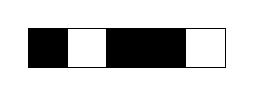
\begin{tikzpicture}
    % X _ X X _
    \foreach \x in {1,2,...,5} {
        \ifnum\x=1 \filldraw[fill=black] (\x*0.5, 0) rectangle (\x*0.5+0.5, -0.5);
        \else\ifnum\x=3 \filldraw[fill=black] (\x*0.5, 0) rectangle (\x*0.5+0.5, -0.5);
        \else\ifnum\x=4 \filldraw[fill=black] (\x*0.5, 0) rectangle (\x*0.5+0.5, -0.5);
        \else \draw (\x*0.5, 0) rectangle (\x*0.5+0.5, -0.5);
        \fi\fi\fi
    }
\end{tikzpicture}
\end{center}

The condition variables will take the following values:
\begin{align*}
c_{00} &= F & c_{01} &= T & c_{02} &= T & c_{03} &= T & c_{04} &= T & c_{05} &= T \\
c_{10} &= F & c_{11} &= F & c_{12} &= F & c_{13} &= F & c_{14} &= T & c_{15} &= T
\end{align*}

A line can be encoded by encoding the puzzle restrictions as follows:
\begin{enumerate}
  \item The most natural rule concerns how to fill in gaps given their sizes.
        In particular, if the $i$-th gap starts at position $s$, then the following $gaps_i - 1$ positions are filled and the position after that is empty.
        Additionally, it's required that the gap hasn't already started being filled and that the previous one has already been completed, which can be expressed using the constraint variables.
        However, there are two exceptions to this rule.
        The first gap does not require the previous gap to be completed and for the last gap not only the cell after, but all cells up to the end (possibly zero) must be empty.
        Only the general rule is presented:
        \begin{center}
          $\forall i, s: \neg c_{i}_{(s+gaps_i-1)} \wedge c_{(i-1)}_{(start-1)} \wedge x_s \implies c_{i}_{(s+gaps_i)} \wedge \bigwedge_{k=s}^{s+gaps_i-1} x_k \wedge \neg x_{s+gaps_i}$
        \end{center}


    \item The previous rule described how to complete a gap, but it doesn't require that that is the only way to do that.
          To fix that, it's required that if a gap is completed by a given cell, then it was either just completed (which can be checked by looking at the values of $x$) or it was already completed by the previous cell.
          \begin{center}
            $\forall i, j \ne 0: c_{i}_{j} \implies c_{i}_{(j-1)} \vee \bigwedge_{k=j-gaps_i}^{j-1} x_k$
          \end{center}

          For cells where the gap could never have ended, a tighter condition can be specified.
          \begin{center}
            $\forall i, j \ne 0: c_{i}_{j} \implies c_{i}_{(j-1)}$
          \end{center}

  \item It has already been specified that for a gap to start being filled in, the previous one should have already been completed. However, it hasn't been specified that if a gap isn't completed, then the next one is not completed as well. In fact, a more strict constraint is included -- if a gap hasn't completed by a position $j$, then the following won't complete at $j$, nor at any position before $j+nextGap$.

  \begin{center}
    $\forall i \ne |gaps|-1, 0 \le k < maxStart(gaps_i): \neg c_i_{(k+gaps_i)} \implies \bigwedge_k^{k+gaps_i+1} \neg c_{(i+1)}_{(j + gaps_{i+1})}$
  \end{center}

  \item If a given gap is completed by position $s$, then it is also completed by position $s+1$.
  \begin{center}
    $\forall i, 0 \le s \le size: (c_i_s \implies c_{(i+1)}_s) $
  \end{center}

  \item Before a gap reaches the minimum position where it can be completed, the completion variables must be false. This represents the start condition.
  \begin{center}
    $\forall i, 0 \le s \le minStart(gaps_i)+gaps_i: \neg c_i_{size}$
  \end{center}

  \item At the end everything should be completed.

  \begin{center}
    $\forall i, c_i_{size}$
  \end{center}
\end{enumerate}

\subsection*{Evaluation}

Even though the second approach was more promising, it could be the case that constants hidden by the $\mathcal{O}$-notation or some heuristics that could only be applied to the first approach made the ``brute-force'' solution more practical.
To understand whether this was the case, a puzzle generator was implemented.
The puzzle size is the sum of the number of rows and columns.
For each puzzle size, 10 puzzles are generated and then both approaches are used to solve it and both the initialization time and the SAT solving time are measured.
The results can be seen in Figure~\ref{fig:bench}. % TODO fix ref

\begin{figure}[H]
  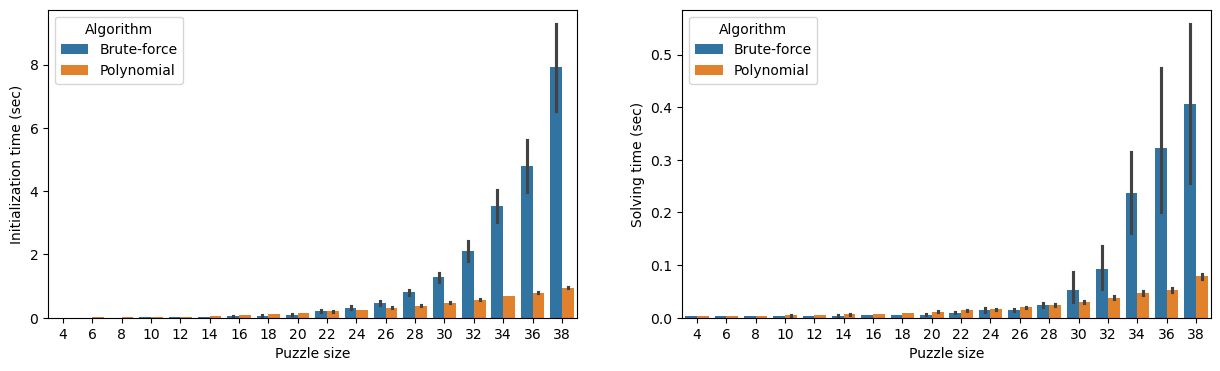
\includegraphics[scale=0.5]{bench.png}
  \centering
  \caption{Execution time for both algorithms proposed}
  \label{fig:bench}
\end{figure}

As can be expected, the polynomial approach is slower for smaller puzzles, but as soon as the puzzle size reaches size 25 it becomes the faster approach.

In addition to this, the percentage of time spent at each state of the process was analysed.
The results of Figure~\ref{fig:util}, show that the initialization time dominates the solving time for all configurations tested but especially for smaller problems.
As mentioned in the lectures, this could be solved by using the C API instead of the Python API for \texttt{z3} -- but this was considered to be out of the scope of this project.

\begin{figure}[H]
  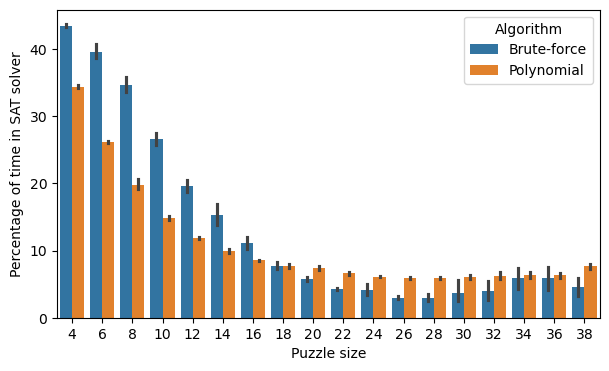
\includegraphics[scale=0.5]{util.png}
  \centering
  \caption{Percentage of time spent in SAT solver}
  \label{fig:util}
\end{figure}

\end{document}
